\subsection{Record Dialogue}
The record dialogue contains two issues, the UI of the dialogue and the functionality to hear your recording.

For the UI, the main issue was an unintuitive icon for recording, discovered by usability tests performed by the previous development group on this product \citep{misc:crocold}. To fix this issue, we decide to make a red circle icon, similar to the look of other recording buttons. Furthermore, the record button changes to a darker colour when recording. 

\begin{figure}[h]
     \centering
     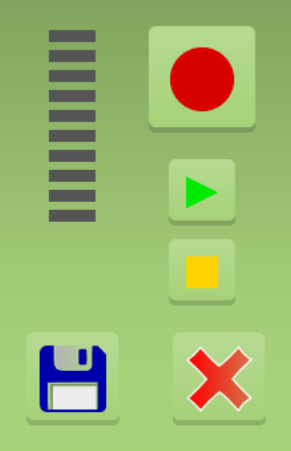
\includegraphics[scale=0.5]{record-dialogue}
     \caption{Record Dialogue window.}
     \label{fig:record-dialogue}
\end{figure}

To get an idea of the dialogue box look, see \figref{fig:record-dialogue}.
As can be seen in the dialogue box, a play and stop button are also added to preview ones recording, which is a feature that was non existent in the program before this sprint.
The functionality of these buttons are implemented with the \textit{SoundPool} android library, which allows for playing of audio.

%preview / stop button
